\documentclass{article}

\usepackage{PRIMEarxiv}

\usepackage[utf8]{inputenc}
\usepackage[T1]{fontenc}
\usepackage{hyperref}
\usepackage{url}
\usepackage{booktabs}
\usepackage{placeins}
\usepackage{amsmath}
\usepackage{amsfonts}
\usepackage{microtype}
\usepackage{fancyhdr}
\usepackage{graphicx}
\usepackage{tikz}
\usepackage{xcolor}

\pagestyle{fancy}
\thispagestyle{empty}
\rhead{ \textit{ }}
\fancyhead[LO]{Measuring the Value of Proxy Oracles in LLM-Based Bug Repair}

\title{Measuring the Value of Proxy Oracles in LLM-Based Bug Repair}

\author{
  Keon Kim \\
  Om Labs \\
  \texttt{keon@omlabs.xyz} \\
  \And
  Krish Chelikavada \\
  Om Labs \\
  \texttt{krish@omlabs.xyz} \\
}

\begin{document}
\maketitle

\begin{abstract}
When an automated repair agent generates multiple plausible patches, how much does a proxy oracle actually help choose the right one? We study this question on SWT-Bench Lite with Jina Test, a repair pipeline built on OpenHands and GPT-5.4. The system generates test candidates and fix candidates, evaluates their cross-product in Docker sandboxes, and selects patches using a deterministic cross-validation (CXV) verdict matrix. Jina Test resolves \textbf{193/276} instances (\textbf{69.9\%}), improving +6.5pp over a single-pass GPT-5.4 baseline.

The main result is a decomposition of where the gain comes from. On a 24-patch selector subset, a naive policy that always chooses fix 0 resolves 11 instances, while CXV selection resolves 13. Resolved instances average 6.0 GOOD\_FAIL verdicts versus 4.0 for unresolved instances, giving a directional selection signal. These findings show that candidate quality is a major driver of end-to-end repair performance and that CXV adds measurable lift on top of a strong pick-first baseline.
\end{abstract}

\keywords{Automated Program Repair \and Cross-Validation \and Software Testing \and LLM Agents \and SWE-bench}

\section{Introduction}

Autonomous software repair agents are evaluated on SWE-bench~\cite{jimenez2024swe} and its variants~\cite{mundler2024swt}, which require generating patches for real GitHub issues. A recurring bottleneck is the \emph{oracle problem}: the agent cannot observe the gold oracle during inference, so it must commit to one patch without verification. Systems that generate multiple candidates and select wisely should outperform single-pass approaches.

The prior e-Otter++ result~\cite{chen2024e} (52.5\%) pioneered this idea by generating 40 fix candidates and using the top-5 as a proxy oracle to filter 10 test candidates. We generalize the approach into a cross-validation (CXV) matrix: K generated tests $\times$ J generated fixes, classified by a 10-verdict regex engine, with frequency-rank selection.

Our system, Jina Test (built on OpenHands 1.16.1~\cite{wang2024openhands}), reaches 69.9\% on SWT-Bench Lite. The selector decomposition shows that \textbf{candidate generation quality is a major source of lift}, with CXV adding a measured selection gain over a pick-first baseline.

\section{Method}

Jina Test applies the following pipeline per instance using GPT-5.4:

\begin{center}
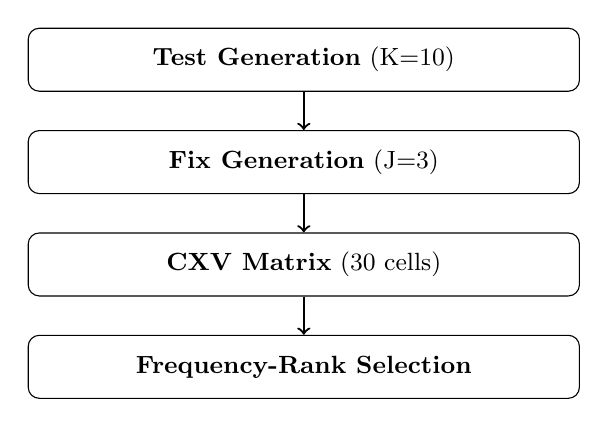
\begin{tikzpicture}[
    box/.style={draw, rounded corners, minimum width=7cm, minimum height=0.8cm, align=center, font=\small},
    arr/.style={->, thick}
]
    \node[box] (s1) at (0, 0)    {\textbf{Test Generation} (K=10)};
    \node[box] (s2) at (0,-1.3)  {\textbf{Fix Generation} (J=3)};
    \node[box] (s3) at (0,-2.6)  {\textbf{CXV Matrix} (30 cells)};
    \node[box] (s4) at (0,-3.9)  {\textbf{Frequency-Rank Selection}};
    \draw[arr] (s1) -- (s2);
    \draw[arr] (s2) -- (s3);
    \draw[arr] (s3) -- (s4);
\end{tikzpicture}
\end{center}

\paragraph{Test Generation.} We generate K=10 test candidates via 5 prompt strategies (direct issue-to-test, snippet-based, assertion-flip, contract-based, exception-focused) at 2 temperatures (0.0, 0.6). Each candidate is evaluated inside a Docker sandbox with the target repository.

\paragraph{Fix Generation.} J=3 fix candidates are generated at temperatures (0.0, 0.5, 1.0) using a dedicated fix-agent prompt through the OpenHands agentic loop. Fixes are extracted as unified diffs.

\paragraph{CXV Matrix.} Each (test$_k$, fix$_j$) pair is evaluated in an isolated sandbox. A 10-verdict regex classifier categorizes the outcome: GOOD\_FAIL (test kills the candidate fix), UNEXPECTED\_PASS (test does not discriminate on buggy code), WRONG\_FAIL (test fails for the wrong reason), and others. The nominal design produces a 30-cell verdict matrix per instance. Let $V_{kj}$ denote the verdict for test candidate $k$ against fix candidate $j$. The discriminative score for test $k$ is
\[
c_k=\sum_{j=1}^{J}\mathbf{1}[V_{kj}=\mathrm{GOOD\_FAIL}].
\]

\paragraph{Selection.} Tests are ranked by $c_k$, normalized frequency score, shorter test diff, and prompt path name. Let $k^\star=\arg\max_k c_k$ after deterministic tie-breaking. After selecting test $k^\star$, the first fix not killed by that test becomes the output patch. If all fixes are killed by the winning test, we choose the fix with the lowest overall kill count. When there is no GOOD\_FAIL signal, the ranking falls through to deterministic tie-breakers and usually returns fix index 0.

\paragraph{Design influences.} Our heterogeneous prompting mirrors e-Otter++'s context masks~\cite{chen2024e}. The assertion-flip strategy draws from AssertFlip~\cite{mundler2024assertflip}. The agentic backbone is OpenHands~\cite{wang2024openhands}, following the paradigm established by SWE-Agent~\cite{yang2024sweagent}.

\section{Experimental Setup}

We evaluate on SWT-Bench Lite~\cite{mundler2024swt} unit-test mode (276 instances). The baseline uses vanilla OpenHands + GPT-5.4 in single-pass mode (J=1). Jina Test is submitted as one prediction set over the full benchmark and uses the CXV pipeline for instances where candidate selection is needed.

All experiments use \texttt{openai/gpt-5.4-2026-03-05}. Verdict classification and selection are deterministic (no LLM). Infrastructure: GCP e2-highmem-16 (16 vCPU, 128GB RAM). Mean execution time: $\sim$788s per instance. The selector decomposition below uses 24 submitted CXV-selected patches with shared candidate sets for pick-first and CXV selection. For each selected instance, CXV evaluates a 30-cell sandbox matrix; verdict classification and selection add no LLM calls beyond candidate generation.

\section{Results}

\begin{table}
\centering
\caption{SWT-Bench Lite unit-test mode (276 instances).}
\small
\begin{tabular}{lrr}
\toprule
\textbf{Method} & \textbf{Resolved} & \textbf{Rate} \\
\midrule
e-Otter++\textsuperscript{\dag} & 145 & 52.5\% \\
Baseline (OpenHands + GPT-5.4) & 175 & 63.4\% \\
\textbf{Jina Test + GPT-5.4}\textsuperscript{\ddag} & \textbf{193} & \textbf{69.9\%} \\
\bottomrule
\end{tabular}
\parbox{0.86\linewidth}{\vspace{0.4em}\footnotesize
\textsuperscript{\dag}Prior published result.
\textsuperscript{\ddag}Jina Test is submitted as a single prediction set.}
\label{tab:main}
\end{table}

\begin{table}
\centering
\caption{Per-repository resolved counts.}
\small
\begin{tabular}{lrr}
\toprule
\textbf{Repository} & \textbf{Baseline} & \textbf{Jina Test} \\
\midrule
django/django & 89 & 96 \\
sympy/sympy & 49 & 55 \\
matplotlib/matplotlib & 6 & 10 \\
sphinx-doc/sphinx & 1 & 2 \\
Others (6 repos) & 30 & 30 \\
\midrule
\textbf{Total} & \textbf{175} & \textbf{193} \\
\bottomrule
\end{tabular}
\label{tab:repos}
\end{table}

Jina Test resolves 18 more instances than the matched GPT-5.4 baseline. The largest absolute gains appear in Django, SymPy, and Matplotlib. Repositories with few failing instances showed no lift, consistent with statistical expectations given J=3 candidates.

\subsection{CXV Signal Quality}

Across 669 recorded CXV cells from the 24-instance selector subset:

\begin{table}
\centering
\caption{CXV verdict distribution (669 cells).}
\small
\begin{tabular}{lrr}
\toprule
\textbf{Verdict} & \textbf{Count} & \textbf{\%} \\
\midrule
UNEXPECTED\_PASS & 250 & 37.4 \\
GOOD\_FAIL & 122 & 18.2 \\
WRONG\_FAIL & 114 & 17.0 \\
Other & 183 & 27.4 \\
\bottomrule
\end{tabular}
\label{tab:verdicts}
\end{table}

GOOD\_FAIL verdicts account for 18.2\% of recorded cells, while 37.4\% of generated tests pass on buggy code (UNEXPECTED\_PASS) and therefore do not discriminate among fixes. This distribution highlights test generation quality as a major factor in proxy-oracle effectiveness.

\subsection{Signal vs. Outcome}

Resolved selector-subset instances averaged 6.0 GOOD\_FAIL verdicts while unresolved instances averaged 4.0:

\begin{table}
\centering
\caption{Selector-subset GOOD\_FAIL signal by final outcome.}
\small
\begin{tabular}{lrr}
\toprule
\textbf{Outcome} & \textbf{Instances} & \textbf{Mean GOOD\_FAIL} \\
\midrule
Resolved & 13 & 6.0 \\
Unresolved & 11 & 4.0 \\
\bottomrule
\end{tabular}
\label{tab:signal-outcome}
\end{table}

The signal is directionally positive. High-signal successes include \texttt{django-16408} (28 GOOD\_FAIL) and \texttt{django-15781} (24), while some high-signal candidates still miss final benchmark requirements. Proxy tests can identify plausible local behavior while still leaving broader-suite correctness to final evaluation.

\subsection{Prompt Strategy Concentration}

All 24 selector-subset instances selected the \texttt{direct} prompt strategy with greedy decoding. The four alternative strategies (snippet, assertflip, contract, exception) never won. This contrasts with e-Otter++~\cite{chen2024e}, which reported large gains (+23.8\% F$\rightarrow$P@10) from heterogeneous prompting. Possible explanations: (a) GPT-5.4's direct test generation may already be strong; (b) our temperature range (0.0, 0.6) may be insufficient to produce meaningfully different candidates; (c) the frequency-rank selector converges quickly to the greedy candidate. This result suggests that heterogeneous test prompting did not drive the selected outputs in this setup; the observed lift comes from the generated candidate set and deterministic selection over the resulting matrix.

\section{Selector Lift}

This is the central question. We decompose performance on the 24-instance selector subset into two components: \emph{fix generation} (producing a candidate set) and \emph{CXV selection} (choosing among those candidates).

For instance $i$, let $f_{ij}$ be fix candidate $j$ and let $Y_i(j)\in\{0,1\}$ indicate whether that candidate resolves the instance under final evaluation. A selector $S$ chooses an index $S(i)$ from the generated candidate set. We compare the generator's default ordering against CXV using
\[
R_{\mathrm{first}}=\frac{1}{n}\sum_{i=1}^{n}Y_i(0),
\qquad
R_{\mathrm{CXV}}=\frac{1}{n}\sum_{i=1}^{n}Y_i(S_{\mathrm{CXV}}(i)).
\]
The realized selector lift is
\[
\Delta_{\mathrm{sel}}=R_{\mathrm{CXV}}-R_{\mathrm{first}}.
\]
This paired comparison separates default candidate quality from the value added by replacing the generator's first candidate with the CXV-selected candidate on the same candidate sets.

\begin{table}
\centering
\caption{CXV selection vs.\ naive baseline (24-instance selector subset).}
\small
\begin{tabular}{lrr}
\toprule
\textbf{Strategy} & \textbf{Resolved/24} & \textbf{Rate} \\
\midrule
Naive (always pick fix 0) & 11 & 45.8\% \\
CXV (frequency-rank) & 13 & 54.2\% \\
\textbf{Realized Selector Lift} & \textbf{+2} & \textbf{+8.4pp} \\
\bottomrule
\end{tabular}
\label{tab:decomposition}
\end{table}

CXV changed the selected fix for \textbf{2 of 13} selector-subset resolved instances (\texttt{django-15781}: fix 0$\rightarrow$1; \texttt{sympy-17022}: fix 0$\rightarrow$2), accounting for the measured +8.4pp selection lift over pick-first.

Because this decomposition covers 24 instances, we treat the measured selector lift as directional evidence rather than a precise estimate of the average benefit of CXV selection.

\paragraph{Takeaway.} CXV improves the pick-first selector baseline from 45.8\% to 54.2\%. For practitioners, \textbf{these results indicate that strong candidate generation likely contributes most of the gain, with deterministic proxy-oracle selection providing incremental benefit when candidate choice is nontrivial}.

\FloatBarrier

\section{Related Work}

Our CXV matrix generalizes e-Otter++'s proxy oracle~\cite{chen2024e}, which filters 10 test candidates against 5 surrogate fixes using binary pass/fail. We build the full K$\times$J matrix with 10-verdict classification. The heterogeneous prompting approach mirrors their context masks. Our assertion-flip strategy draws from AssertFlip~\cite{mundler2024assertflip}. The agentic backbone is OpenHands~\cite{wang2024openhands}, following the paradigm established by SWE-Agent~\cite{yang2024sweagent}. Multi-candidate generation relates to self-consistency~\cite{wang2023selfconsistency} and best-of-N sampling. The test-as-oracle concept connects to mutation testing~\cite{demillo1978hints}, GenProg~\cite{le2012genetic}, and feedback-directed test generation~\cite{pacheco2007feedback}.

\section{Conclusion}

We presented a cross-validation proxy oracle for LLM-based bug repair, reaching 69.9\% on SWT-Bench Lite (+6.5pp over a matched GPT-5.4 baseline). The results suggest that \textbf{candidate generation quality is a major driver of repair performance in this setup, while CXV provides a modest but measurable lift over pick-first selection on the analyzed subset}. On the 24-instance selector decomposition, CXV selection adds 8.4pp on top of a naive pick-first strategy, including two resolved cases that require a non-default fix choice. This work is an integration and empirical contribution: it combines best-of-N generation, cross-validation, and deterministic test-based filtering into a concrete repair pipeline, then decomposes the resulting selector behavior. For future work, improving test generation quality and exploring larger J with cheaper models are natural next steps.

\bibliographystyle{unsrt}
\bibliography{references}

\end{document}
